\documentclass[11pt,letterpaper]{article}
\usepackage[lmargin=1in,rmargin=1in,tmargin=1in,bmargin=1in]{geometry}
\usepackage{../style/homework}
\usepackage{../style/commands}
\setbool{quotetype}{true} % True: Side; False: Under
\setbool{hideans}{true} % Student: True; Instructor: False

% -------------------
% Content
% -------------------
\begin{document}

\homework{6: Due 11/04}{I used to sell furniture for a living. The trouble was, it was my own.}{Les Dawson}

% Problem 1
\problem{10} As accurately as possible, sketch the feasible region given by the following maximization problem:
	\[
	\begin{aligned}
	z&= 4x_1 + 6x_2 \\
	x_1 + x_2&\leq 10 \\
	2x_1 - x_2&\geq 2 \\
	x_1, x_2&\geq 0
	\end{aligned}
	\]
Is this region bounded or unbounded?



% Problem 2
\problem{10} As accurately as possible, sketch the feasible region given by the following maximization problem:
	\[
	\begin{aligned}
	z&= x_1 - 3x_2 \\
	x_1 + x_2&\geq 4 \\
	\frac{1}{2}\,x_1 + 3x_2&\geq 7 \\
	x_1, x_2&\geq 0
	\end{aligned}
	\]
Is this region bounded or unbounded?


% Problem 3
\problem{10} Find a system of inequalities that gives the following feasible region:
	\[
	\fbox{
	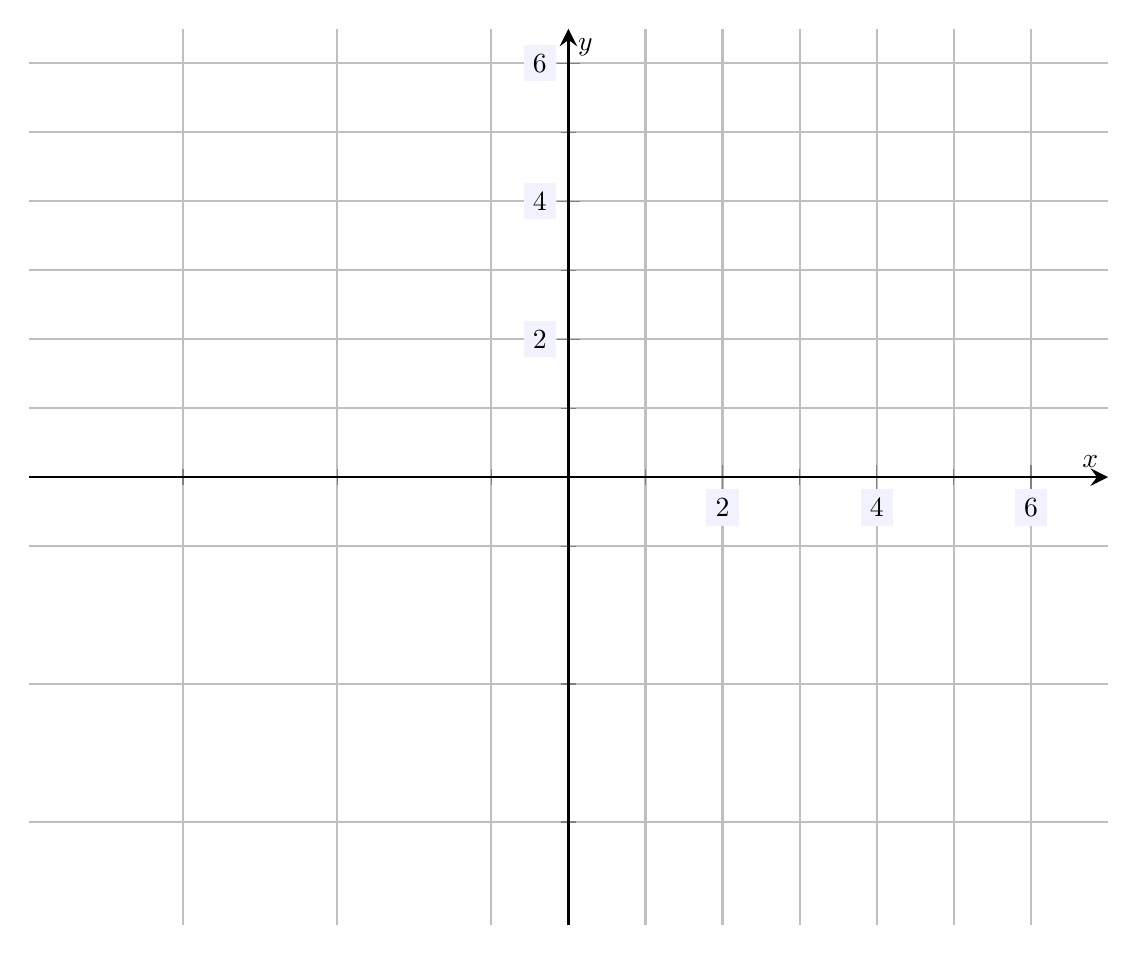
\begin{tikzpicture}[scale=2,every node/.style={scale=0.5}]
	\begin{axis}[
	grid=both,
	axis lines=middle,
	ticklabel style={fill=blue!5!white},
	xmin= -7, xmax=7,
	ymin= -6.5, ymax=6.5,
	xtick={0,2,4,6,8,10},
	ytick={0,2,4,6,8,10},
	minor tick = {-5,-3,...,5},
	xlabel=\(x\),ylabel=\(y\),
	]
	\end{axis}
	\end{tikzpicture}
	}
	\]












\end{document}